\documentclass[10pt, dvipsnames]{beamer}

\usepackage[english,main=russian]{babel}
\usepackage{textpos}
\usepackage{graphicx}
\usepackage{amsmath}
\usepackage{kbordermatrix}
\usepackage{qtree}
\usepackage{ulem}
\usepackage{color}
\usepackage{textcomp}
\usepackage{relsize}
\usepackage{tikz}
\usetikzlibrary{shapes.geometric}
\usetikzlibrary{arrows.meta,arrows}

\graphicspath{ {./images/} }

\usepackage{amsmath}
\makeatletter
\renewcommand*\env@matrix[1][\arraystretch]{%
  \edef\arraystretch{#1}%
  \hskip -\arraycolsep
  \let\@ifnextchar\new@ifnextchar
  \array{*\c@MaxMatrixCols c}}
\makeatother

\title{A Quantitative Study of Two Matrix Clustering Algorithms}
\author{{Александр Слесарев}%\inst{1}
		\\
		студент СПбГУ, 2-й курс\\[0.1cm]
		Вячеслав Галактионов,\;%\inst{1,2}
		Никита Бобров,\;%\inst{1,2}
		Георгий Чернышев%\inst{1,2}
		\\
		СПбГУ, JetBrains Research
		}
		
\date[SEIM 2019]{SEIM 2019\\ 13 апреля 2019}

\begin{document}

\maketitle

\begin{frame}{Типы фрагментирования}
	\begin{itemize}
	\item Горизонтальное фрагментирование\\[0.4cm]
	\item Вертикальное фрагментирование\\[0.4cm]
	\item Гибридное фрагментирование\\[0.4cm]
	\end{itemize}
\end{frame}

\begin{frame}{Число возможных фрагментов}
	\begin{columns}
		\begin{column}{0.5\textwidth}
			\begin{textblock}{10}(-0.8,-4)
Число Белла -- число всех неупорядоченных разбиений $n$-элементного множества 
\\[0.5cm]
При больших $n$ выполняется $B(n) \approx n^{n}$,\newline например, $B(30) \approx 10^{23}$
			\end{textblock}
		\end{column}
		\begin{column}{0.2\textwidth}
			\begin{tabular}{|c|c|}
				\hline
				$n$ & $B(n)$\\ \hline
				1   & 1     \\ \hline
				2   & 1     \\ \hline
				3   & 2     \\ \hline
				4   & 5     \\ \hline
				5   & 15    \\ \hline
				6   & 52    \\ \hline
				7   & 203   \\ \hline
				8   & 877   \\ \hline
				9   & 4140  \\ \hline
			   10   & 21147 \\ \hline
			   11  & 115975 \\ \hline
			\end{tabular}
		\end{column}
	\end{columns}	
\end{frame}

\begin{frame}{Виды вертикального фрагментирования}	
	\begin{itemize}
	\item стоимостное\\[0.4cm] 
	\item эвристическое\\[0.2cm]
		\begin{itemize}
		\item \color{red}\uline{\color{black}{методы матричной кластеризации}}\color{black}\\[0.1cm]
		\item графовый подход\\[0.1cm]
		\item data mining 
		\end{itemize}
	\end{itemize}
\end{frame}

\begin{frame}{О проекте}
Цель: экспериментальная проверка алгоритмов ВФ на основе подхода матричной кластеризации\\[0.1cm]
Современные работы по ВФ на матричной кластеризации:	
	\begin{itemize}
	\item C. Cheng “Algorithms for vertical partitioning in database physical design”,\,$\bold{1993}$
	\item C.-H. Cheng “A branch and bound clustering algorithm”,\,$\bold{1995}$
	\item C.-H. Cheng and J. Motwani “An examination of cluster
identification-based algorithms for vertical partitions”,\,$\bold{2009}$
	\item C.-H. Cheng et al. “An improved branch-and-bound clustering approach for data partitioning”,\,$\bold{2011}$
	\end{itemize}

Наши предыдущие работы:
	\begin{itemize}
	\item V. Galaktionov et al. “Matrix clustering algorithms for vertical partitioning problem: an initial performance study”,\,$\bold{2016}$
	\item V. Galaktionov “Parallelization of matrix clustering algorithms”,\,$\bold{2016}$
	\item V. Galaktionov et al. “A study of several matrix-clustering vertical partitioning algorithms in a disk-based environment”,\,$\bold{2017}$
	\end{itemize}
\end{frame}

\begin{frame}{Матрица запросов}
	\begin{textblock}{13}(2,-4)
		\begin{flushleft}
q1: SELECT a FROM T WHERE a > 10;\\
q2: SELECT b, f FROM T;\\
q3: SELECT a, c FROM T WHERE a = c;\\
q4: SELECT a FROM T WHERE a < 10;\\
q5: SELECT e FROM T;\\
q6: SELECT d, e FROM T WHERE d + e > 0;\\
		\end{flushleft}
	\end{textblock}
	\begin{textblock}{13}(-4,1.5)
\[
  \kbordermatrix{
        & a & b & c & d & e & f \\
    q_1 & 1 & 0 & 0 & 0 & 0 & 0 \\
    q_2 & 0 & 1 & 0 & 0 & 0 & 1 \\
    q_3 & 1 & 0 & 1 & 0 & 0 & 0 \\
    q_4 & 1 & 0 & 0 & 0 & 0 & 0 \\
    q_5 & 0 & 0 & 0 & 0 & 1 & 0 \\
    q_6 & 0 & 0 & 0 & 1 & 1 & 0
  }
\]
	\end{textblock}

	\begin{textblock}{13}(4,1.5)
\[
  \kbordermatrix{
        & a & c & b & f & d & e \\
    q_1 & 1 & 0 & 0 & 0 & 0 & 0 \\
    q_3 & 1 & 1 & 0 & 0 & 0 & 0 \\
    q_4 & 1 & 0 & 0 & 0 & 0 & 0 \\
    q_2 & 0 & 0 & 1 & 1 & 0 & 0 \\
    q_6 & 0 & 0 & 0 & 0 & 1 & 1 \\
    q_5 & 0 & 0 & 0 & 0 & 0 & 1
  }
\]
	\end{textblock}
	
	\begin{textblock}{1}(0,-10)
		\begin{tikzpicture}[overlay,remember picture]
	\draw[-Latex] (4.4,-8.7) -- (6,-8.7);

	\draw [color=red] (7.13,-7.38) rectangle (8.15,-8.65);
	\draw [color=red] (8.15,-8.65) rectangle (9.15,-9);
	\draw [color=red] (9.15,-9) rectangle (10.2,-9.93);
	
		\end{tikzpicture}
	\end{textblock}
\end{frame}

\begin{frame}{Cluster identification}
	\begin{columns}	
	\renewcommand{\arraystretch}{0.9}
	\begin{column}{0.4\textwidth}
\[
\tiny
  \kbordermatrix{
      & 1 & 2 & 3 & 4 & 5 & 6 \\
    1 & 0 & 1 & 1 & 1 & 0 & 0 \\
    2 & 1 & 0 & 0 & 0 & 1 & 0 \\
    3 & 1 & 0 & 0 & 0 & 1 & 0 \\
    4 & 0 & 0 & 1 & 1 & 0 & 1 \\
    5 & 0 & 1 & 1 & 1 & 0 & 1 \\
  }
\]
	\end{column}

	\begin{column}{0.4\textwidth}
\[
\tiny
  \kbordermatrix{
      &        1  &        2  &        3  &        4  &        5  &        6  \\
    1 & \alert{0} & \alert{1} & \alert{1} & \alert{1} & \alert{0} & \alert{0} \\
    2 &        1  & \alert{0} & \alert{0} & \alert{0} &        1  &        0  \\
    3 &        1  & \alert{0} & \alert{0} & \alert{0} &        1  &        0  \\
    4 & \alert{0} & \alert{0} & \alert{1} & \alert{1} & \alert{0} & \alert{1} \\
    5 & \alert{0} & \alert{1} & \alert{1} & \alert{1} & \alert{0} & \alert{1} \\
  }
\]
	\end{column}

	\begin{column}{0.4\textwidth}
\[
\tiny
  \kbordermatrix{
      & 1 & 2 & 3 & 4 & 5 & 6 \\
    1 & 0 & 1 & 1 & 1 & 0 & 0 \\
    2 & 1 & 0 & 0 & 0 & 1 & 0 \\
    3 & 1 & 0 & 0 & 0 & 1 & 0 \\
    4 & 0 & 0 & 1 & 1 & 0 & 1 \\
    5 & 0 & 1 & 1 & 1 & 0 & 1 \\
  }
\]
	\end{column}
	\end{columns}
	
	\begin{center}
\[
  \kbordermatrix{
      & 2 & 3 & 4 & 6 & 1 & 5 \\
    1 & 1 & 1 & 1 & 0 & 0 & 0 \\
    4 & 0 & 1 & 1 & 1 & 0 & 0 \\
    5 & 1 & 1 & 1 & 1 & 0 & 0 \\
    2 & 0 & 0 & 0 & 0 & 1 & 1 \\
    3 & 0 & 0 & 0 & 0 & 1 & 1 \\
  }
\]
	\end{center}	
	
\begin{textblock}{1}(0,-10)
	\begin{tikzpicture}[overlay,remember picture]
	\draw[-Latex] (3,-1.8) -- (3.8,-1.8);
	\draw[-Latex] (7.3,-1.8) -- (8.1,-1.8);

	\path (0.1,-1.45) edge[dashed] (2.8,-1.45);
	\path (1.645,-2.4) edge[dashed] (1.645,-1);
	\path (1.21,-2.4) edge[dashed] (1.21,-1);
	\path (0.76,-2.4) edge[dashed] (0.76,-1);
	
	\pgfmathsetmacro{\movefst}{4.31}

	%\path (0.1 + \movefst,-1.45) edge[dashed] (2.8 + \movefst,-1.45);
	%\path (1.645 + \movefst,-2.4) edge[dashed] (1.645 + \movefst,-1);
	%\path (1.21 + \movefst,-2.4) edge[dashed] (1.21 + \movefst,-1);
	%\path (0.76 + \movefst,-2.4) edge[dashed] (0.76 + \movefst,-1);
	%\path (0.1 + \movefst,-2.2) edge[dashed] (2.8 + \movefst,-2.2);
	%\path (0.1 + \movefst,-2) edge[dashed] (2.8 + \movefst,-2);

	\path (0.1 + 2*\movefst,-1.45) edge[dashed] (2.8 + 2*\movefst,-1.45);
	\path (1.645 + 2*\movefst,-2.4) edge[dashed] (1.645 + 2*\movefst,-1);
	\path (1.21 + 2*\movefst,-2.4) edge[dashed] (1.21 + 2*\movefst,-1);
	\path (0.76 + 2*\movefst,-2.4) edge[dashed] (0.76 + 2*\movefst,-1);
	\path (0.1 + 2*\movefst,-2.2) edge[dashed] (2.8 + 2*\movefst,-2.2);
	\path (0.1 + 2*\movefst,-2) edge[dashed] (2.8 + 2*\movefst,-2);
	\path (2.55 + 2*\movefst,-2.4) edge[dashed] (2.55 + 2*\movefst,-1);

	\end{tikzpicture}
\end{textblock}

\end{frame}

\begin{frame}{Поиск решения -- 1}
$M$ -- матрица запросов\\[0.2cm]	
$M_i^j$ -- $i$-й узел на $j$-ом уровне фрагментирования\\[0.4cm] 
\Tree[.$M$ [.$M_1^1$ [.$M_1^2$ ]
                     [.$M_2^2$ ]]
           [.$M_2^1$ [.$M_3^2$ ]
                     [.$M_4^2$ ]
                     [.$M_5^2$ [.$M_1^3$ ]
                     		   [.$M_2^3$ ]
                               [.$M_3^3$ ]]
                     [.$M_6^2$ ]]]
                                                 
\end{frame}

\begin{frame}{Поиск решения -- 2}
	\begin{textblock}{13}(0.7,-4)
		\begin{columns}
			\begin{column}{0.47\textwidth}
	$R$ - множество индексов транзакций $M$\\[0.2cm]
	$C$ - множество индексов атрибутов $M$
			\end{column}
			\begin{column}{0.6\textwidth}
	$cohesion(M) = \displaystyle\frac{|\{a_{ij} = 1, i \in R \land j \in C\}|}{|R|*|C|}$
			\end{column}
		\end{columns}
	\end{textblock}
	\begin{textblock}{13}(0,2)
	Набор кластеров - решение, если каждый кластер $S$ удовлетворяет условиям: 
		\begin{itemize}
		\item $cohesion(S) < threshold$
		\item В $S$ отсутствуют нулевые строки или столбцы
		\end{itemize} 
	\end{textblock}
\end{frame}

%\begin{frame}{Метод ветвей и границ 2009 -- 2}
%	\begin{itemize}
%	\item $Q_j = \{j'\neq j:a_{ij'} = 1 \land \exists i : a_{ij} = 1\}$
%	\item $C_j = Q_j \cup \{j\}$
%	\item $R_j = \{i:a_{ij} = 1 \land \exists j' \in C_j : a_{ij'} = 1\}$
%	\item $void\_measure(attribute) = |\{a_{ij'} = 0,\;i \in R_j \land j' \in C_j \}|$
%	\end{itemize}	
%\end{frame}

\begin{frame}{Метод ветвей и границ 2009 -- 1}	
%\begin{itemize}
%	\item (инициализация) дерево состоит из корневого узла с матрицей транзакций в нем, $Z_U = \infty$
%	\item (ветвление) находим в матрице текущего узла подматрицу $S : cohesion(S) < threshold$
%	\item (выбор решения) у каждого нового узла обновляем $Z_L$; убираем узел из рассмотрения, если:
%		\begin{enumerate}
%			\item $Z_L \geq Z_U$
%			\item какая-то из полученных подматриц содержит пустые строки/столбцы
%		\end{enumerate}
%	\item (завершение фрагментирования) в случае, если не осталось узлов для выбора решения, возвращаем текущее решение, иначе начинаем ветвление
%	\end{itemize}
	\begin{textblock}{13}(0,-5.5)
нижняя граница: $Z_L$ -- число единиц, удаленных из матрицы транзакции в ходе ветвления\\[0.1cm]
верхняя граница: $Z_U$ -- минимальный $Z_L$ среди найденных решений\\[0.2cm]
	\end{textblock}
	
	\begin{textblock}{1}(1,0.4) 
\[
\small
  \kbordermatrix{
      & 1 & 2 & 3 & 4 & 5 \\
    1 & 1 & 1 & 0 & 0 & 0 \\
    2 & 1 & 1 & 1 & 1 & 1 \\
    3 & 0 & 0 & 0 & 1 & 1 \\
    4 & 0 & 0 & 0 & 1 & 1 \\
  }
\]
	\end{textblock}

	\begin{textblock}{1}(0,4.3)
\small void measures
	\end{textblock}

	\begin{textblock}{1}(1.7,4.7)
\mbox{\small\hspace{7pt}3\hspace{10pt}3\hspace{10pt}0\hspace{10pt}6\hspace{10pt}6}
	\end{textblock}

	\begin{textblock}{1}(8,-3.6)
\[
\small
  \kbordermatrix{
      & 1 & 2 & 3 & 4 & 5 \\
    1 & 1 & 1 & 0 & 0 & 0 \\
    2 & 1 & 1 & 1 & * & 1 \\
    3 & 0 & 0 & 0 & 1 & 1 \\
    4 & 0 & 0 & 0 & 1 & 1 \\
  }
\]
	\end{textblock}

	\begin{textblock}{1}(8,0.4)
\[
\small
  \kbordermatrix{
      & 1 & 2 & 3 & 4 & 5 \\
    1 & 1 & 1 & 0 & 0 & 0 \\
    2 & 1 & 1 & 1 & 1 & 1 \\
    3 & 0 & 0 & 0 & * & 1 \\
    4 & 0 & 0 & 0 & 1 & 1 \\
  }
\]
	\end{textblock}

	\begin{textblock}{1}(8,4.4)
\[
\small
  \kbordermatrix{
      & 1 & 2 & 3 & 4 & 5 \\
    1 & 1 & 1 & 0 & 0 & 0 \\
    2 & 1 & 1 & 1 & 1 & 1 \\
    3 & 0 & 0 & 0 & 1 & 1 \\
    4 & 0 & 0 & 0 & * & 1 \\
  }
\]
	\end{textblock}
	
	\begin{textblock}{1}(0,-10)
		\begin{tikzpicture}[overlay,remember picture]
		\draw[-Latex] (4.5,-7.5) -- (6.2,-5.2);
		\draw[-Latex] (4.5,-7.7) -- (6.2,-7.7);
		\draw[-Latex] (4.5,-7.9) -- (6.2,-10.2);
		\end{tikzpicture}
	\end{textblock}

%	\begin{figure}
%Иллюстрация правила ветвления
%		\includegraphics[scale=0.2]{8.png}	
%	\end{figure}
\end{frame}

\begin{frame}{Метод ветвей и границ 2009 -- 2}
Распределение межкластерных элементов по матрицам в решении:
	\begin{itemize}
	\item (separate) составить отдельный фрагмент из межкластерных эелементов
	\item (nearest) добавить межкластерный столбец в тот фрагмент, где есть какая-то его часть
	\item (replicate) добавить в каждый фрагмент все необходимые межкластерные столбцы
	\end{itemize}
\end{frame}

\begin{frame}{Метод ветвей и границ 2011 -- 1}
	\begin{textblock}{13}(0,-5.5)
нижняя граница: $Z_L$ -- глубина узла в дереве\\[0.1cm]
верхняя граница: $Z_U$ -- минимальный $Z_L$ среди найденных решений\\[0.2cm]
	\end{textblock}
	
	\begin{textblock}{1}(1,0.6)
\[
\tiny
  \kbordermatrix{
      & 1 & 2 & 3 & 4 & 5 \\
    1 & 0 & 1 & 1 & 1 & 0 \\
    2 & 1 & 0 & 0 & 0 & 1 \\
    3 & 1 & 0 & 0 & 0 & 1 \\
    4 & 0 & 0 & 1 & 1 & 0 \\
  }
\]	
	\end{textblock}

	\begin{textblock}{1}(0.5,3.5)
\tiny void measures
	\end{textblock}

	\begin{textblock}{1}(1.5,3.6)
\mbox{\tiny\hspace{7pt}3\hspace{9pt}3\hspace{10pt}0\hspace{10pt}6\hspace{9pt}6}
	\end{textblock}
	
	\begin{textblock}{1}(0,-10)
		\begin{tikzpicture}[overlay,remember picture]
		\draw[-Latex] (4,-7.3) -- (6.6,-4.5);
		\draw[-Latex] (4,-7.4) -- (6.6,-6);
		\draw[-Latex] (4,-7.5) -- (6.6,-7.5);
		\draw[-Latex] (4,-7.6) -- (6.6,-9);
		\draw[-Latex] (4,-7.7) -- (6.6,-10);
		\end{tikzpicture}
	\end{textblock}
	
	\begin{textblock}{1}(9,-4.4)
\[
\tiny
  \kbordermatrix{
      & 1 & 2 & 3 & 4 & 4` & 4`` & 5 \\
    1 & 1 & 1 & 0 & 0 & 0  & 0   & 0 \\
    2 & 1 & 1 & 1 & 1 & 0  & 0   & 1 \\
    3 & 0 & 0 & 0 & 0 & 1  & 0   & 1 \\
    4 & 0 & 0 & 0 & 0 & 0  & 1   & 1 \\
  }
\]
	\end{textblock}

	\begin{textblock}{1}(9,-1.8)
\[
\tiny
  \kbordermatrix{
      & 1 & 2 & 3 & 4 & 5 & 5` & 5`` \\
    1 & 1 & 1 & 0 & 0 & 0 & 0  & 0   \\
    2 & 1 & 1 & 1 & 1 & 1 & 0  & 0   \\
    3 & 0 & 0 & 0 & 1 & 0 & 1  & 0   \\
    4 & 0 & 0 & 0 & 1 & 0 & 0  & 1   \\
  }
\]
	\end{textblock}

	\begin{textblock}{1}(9,0.6)
\[
\tiny
  \kbordermatrix{
      & 1 & 1` & 2 & 3 & 4 & 5 \\
    1 & 1 & 0  & 1 & 0 & 0 & 0 \\
    2 & 0 & 1  & 1 & 1 & 1 & 1 \\
    3 & 0 & 0  & 0 & 0 & 1 & 1 \\
    4 & 0 & 0  & 0 & 0 & 1 & 1 \\
  }
\]
	\end{textblock}

	\begin{textblock}{1}(9,3)
	\[
\tiny
  \kbordermatrix{
      & 1 & 2 & 2` & 3 & 4 & 5 \\
    1 & 1 & 1 & 0  & 0 & 0 & 0 \\
    2 & 1 & 0 & 1  & 1 & 1 & 1 \\
    3 & 0 & 0 & 0  & 0 & 1 & 1 \\
    4 & 0 & 0 & 0  & 0 & 1 & 1 \\
  }
\]
	\end{textblock}

	\begin{textblock}{1}(9,5.4)
	\[
\tiny
  \kbordermatrix{
      & 1 & 2 & 3 & 4 & 5 \\
    1 & 1 & 1 & 0 & 0 & 0 \\
    2 & 1 & 1 & 1 & 1 & 1 \\
    3 & 0 & 0 & 0 & 1 & 1 \\
    4 & 0 & 0 & 0 & 1 & 1 \\
  }
\]
	\end{textblock}

%	\begin{figure} 
%		\begin{textblock}{13}(-1,-2)
%Иллюстрация правила ветвления
%		\includegraphics[scale=0.2]{11.png}
%		\end{textblock}
%	\end{figure}
\end{frame}

\begin{frame}{Метод ветвей и границ 2011 -- 2}
	\begin{textblock}{13}(0,-5.5)
Постобработка решения
	\end{textblock}
	
	\begin{textblock}{1}(0,-10)
		\begin{tikzpicture}[overlay,remember picture]
		\draw[-Latex] (4.8,-4.5) -- (4.8,-5.2);
		
		\draw[-Latex] (4.8,-6.5) -- (3.3,-7);
		\draw[-Latex] (4.8,-6.5) -- (5.5,-7);
		\draw[-Latex] (4.8,-6.5) -- (7,-7);
		
		\draw[-Latex] (3.2,-8) -- (3.2,-8.7);
		
		\draw[-Latex] (5.7,-7.8) -- (6.5,-8.7);
		\draw[-Latex] (7.6,-7.8) -- (6.7,-8.7);
		\end{tikzpicture}
	\end{textblock}

	\begin{textblock}{1}(4,-5)
\[
\tiny
  \kbordermatrix{
      & 1 & 2 & 3 & 4 & 5 \\
    1 & 1 & 1 & 0 & 0 & 0 \\
    2 & 1 & 1 & 1 & 1 & 1 \\
    3 & 0 & 0 & 0 & 1 & 1 \\
    4 & 0 & 0 & 0 & 1 & 1 \\
  }
\]
	\end{textblock}
	
	\begin{textblock}{1}(2.9,-1.8)
\[
\tiny
  \kbordermatrix{
      & 1 & 2 & 3 & 4 & 4` &  4`` & 5 & 5` & 5`` \\
    1 & 1 & 1 & 0 & 0 & 0  &  0   & 0 & 0  & 0   \\
    2 & 1 & 1 & 1 & 1 & 0  &  0   & 1 & 0  & 0   \\
    3 & 0 & 0 & 0 & 0 & 1  &  0   & 0 & 1  & 0   \\
    4 & 0 & 0 & 0 & 0 & 0  &  1   & 0 & 0  & 1   \\
  }
\]
	\end{textblock}
	
	\begin{textblock}{1}(2,1.4)
\[
\tiny
  \kbordermatrix{
	  & 1 & 2 & 3 & 4 & 5 \\
	1 & 1 & 1 & 0 & 0 & 0 \\
    2 & 1 & 1 & 1 & 1 & 1 \\
  }
\]
	\end{textblock}
	
	\begin{textblock}{1}(6,1.4)
\[
\tiny
  \kbordermatrix{
	  & 4 & 5 \\
	3 &	1 & 1 \\
  }
\]
	\end{textblock}
	
	\begin{textblock}{1}(8.5,1.4)
\[
\tiny
  \kbordermatrix{
	  & 4 & 5 \\
	4 &	1 & 1 \\
  }
\]
	\end{textblock}
	
	\begin{textblock}{1}(2,4)
\[
\tiny
  \kbordermatrix{
	  & 1 & 2 & 3 & 4 & 5 \\
	1 & 1 & 1 & 0 & 0 & 0 \\
    2 & 1 & 1 & 1 & 1 & 1 \\
  }
\]
	\end{textblock}
	
	\begin{textblock}{1}(7.1,4)
\[
\tiny
  \kbordermatrix{
      & 4 & 5 \\
	3 & 1 & 1 \\
	4 &	1 & 1 \\
  }
\]
	\end{textblock}

%	\begin{figure}
%		\begin{textblock}{13}(-1.2,-3)
%		Постобработка решения
%		\includegraphics[scale=0.23]{12.png}
%		\end{textblock}
%	\end{figure} 
\end{frame}

\begin{frame}{Тестовый стенд}
	\begin{textblock}{5}(0,-5.5)
Структура программы
	\end{textblock}
	
	\begin{textblock}{1}(0,-5.5)
		\begin{tikzpicture}[overlay,remember picture]
\draw (1.5,-1.3) rectangle (8.5,-4.5);

\draw (2,-1.04) node[rectangle, draw, fill=gray]{vpart};

\draw (0.3,-2) node[rectangle, draw, fill=gray]{workload};
\draw[-Latex] (1.05,-2) -- (1.95,-2);
\draw (2.5,-2) node[rectangle, draw, fill=gray]{parser};
\draw[-Latex] (3.05,-2) -- (6.77,-2);
\draw[-Latex] (2.5,-2.23) -- (2.5,-3.71);
\draw (7.5,-2) node[rectangle, draw, fill=gray]{executor};
\draw[latex'-latex'] (8.23,-2) -- (9.34,-3);

\draw (5,-3) node[rectangle, draw, fill=gray]{rewriter};
\draw[-Latex] (5.67,-3) -- (6.77,-2.2);
\draw (10.3,-3) node[rectangle, draw, fill=gray]{PostgreSQL};

\draw (2.7,-4) node[rectangle, draw, fill=gray]{algorithm};
\draw[-Latex] (3.5,-3.9) -- (4.34,-3);
\draw[-Latex] (3.5,-4) -- (6.47,-4);
\draw (7.35,-4) node[rectangle, draw, fill=gray]{partitioner};
\draw[-Latex] (6.48,-3.9) -- (5.67,-3);
\draw[-Latex] (8.23,-4) -- (9.32,-3);
		\end{tikzpicture}
	\end{textblock}
	
	\begin{textblock}{10}(0,3)
Критерии оценки алгоритмов\,:
		\begin{itemize}
		\item скорость кластеризации
		\item скорость выполнения запросов после применения алгоритма
		\item затраты памяти на хранение кластеров
		\end{itemize}
	\end{textblock}
	
%	\begin{figure}
%		\begin{textblock}{13}(-0.8,-3)
%		Структура программы
%		\includegraphics[scale=0.36]{14.png}
%		\end{textblock}
%	\end{figure}
\end{frame}


\begin{frame}{Реализация}
	\begin{textblock}{10}(0,-5.5)
Аппаратные средства\,:
		\begin{itemize}
		\item Inspiron 15 7000 Gaming (0798)
		\item 8GiB RAM
		\item Intel(R)
Core(TM) i5-7300HQ\\ CPU @ 2.50GHz
		\item TOSHIBA 1TB MQ02ABD1
		\end{itemize}
	\end{textblock}
	
	\begin{textblock}{10}(0,0)
Программное обеспечение\,:	
		\begin{itemize}
		\item Ubuntu 18.10
		\item PostgreSQL 11.1
		\item gcc 8.2.0
		\end{itemize}
	\end{textblock}
	
	\begin{textblock}{10}(0,4)
Датасет\,:
		\begin{itemize}
		\item SDSS Star table
		\end{itemize}
	\end{textblock}
\end{frame}

\begin{frame}{Обеспечение чистоты экспериментов}	
	\begin{textblock}{1}(2,-4.7)
$$\mathlarger{\sum}_{q_i \in Queries} \frac{size(T)}{time(q_i, T)} = \mathlarger{\sum}_{q_i \in Queries} \frac{size(table(q_i))}{time(q_i, table(qi))}$$	
	\end{textblock}
	
	\begin{textblock}{15}(0,-1)
$size(T)$ -- размер исходной таблицы в байтах\\
$size(table(q_i))$ -- размер фрагмента, соответствующего запросу\\
$time(q_i, table)$ -- время выполнения запроса к соответствующей таблице
	\end{textblock}
	
	\begin{textblock}{10}(0,2)
		\begin{itemize}
		\item сбросить системный кеш\,: установить флаг $3$ в \path{/proc/sys/vm/drop_caches}
		\item запретить параллельное выполнение запросов\,: set 
max\_parallel\_workers\_per\_gather \ to \ 0\,;
		\end{itemize}
	\end{textblock}
\end{frame}

\begin{frame}{Эксперимент 1 -- затраты памяти на фрагменты}
	\begin{itemize}
	\item база данных SDSS-IV Data Release 14, 2016
	\item 8 запросов
	\item таблица "Star"
	\item 509 атрибутов, 492515 записей
	\item каждое показание является средним значением из 10 итерациий
	\end{itemize}
	\begin{figure}[t]
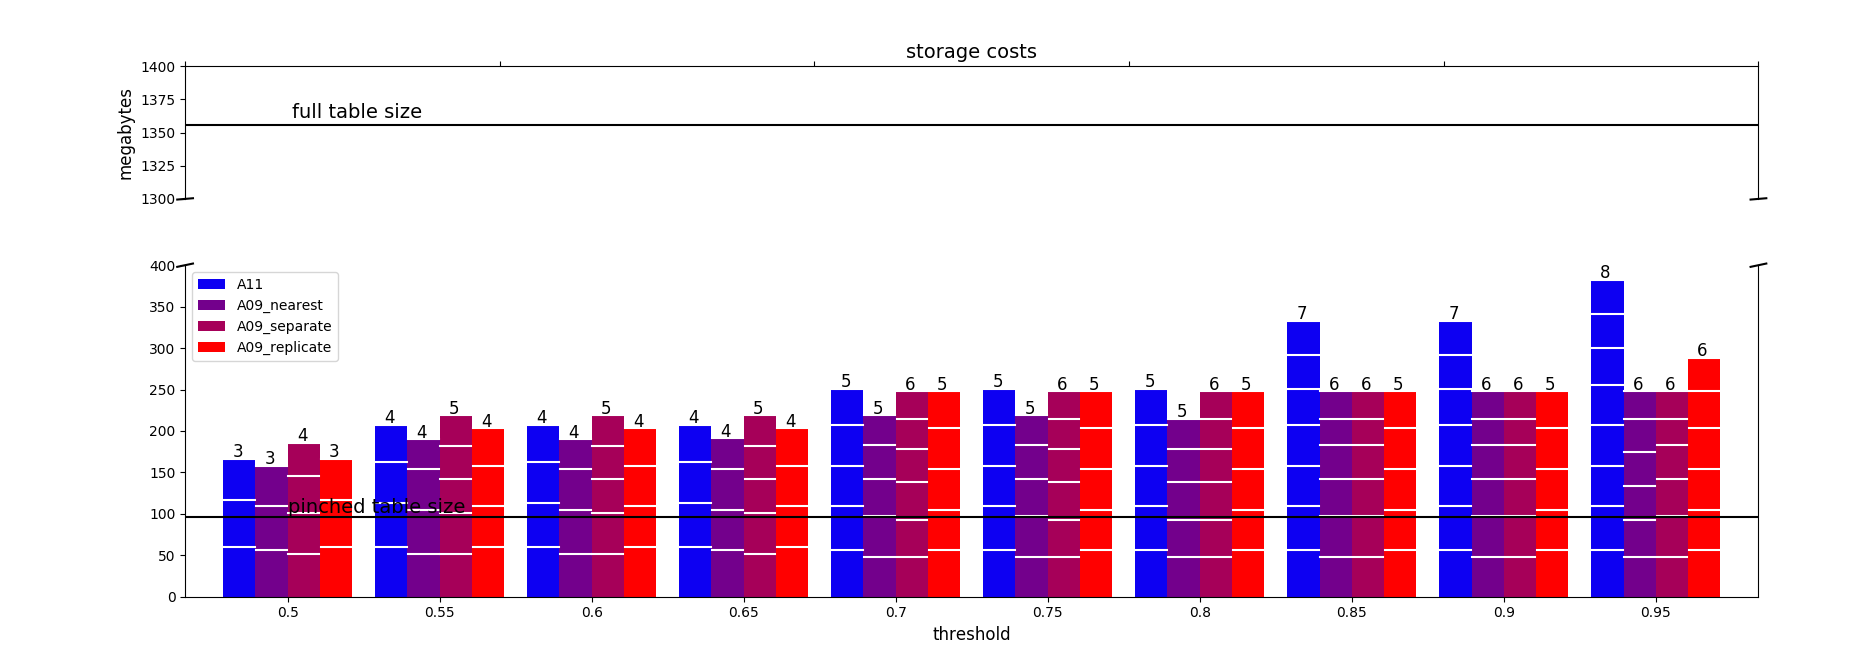
\includegraphics[width=\textwidth]{./images/A11-vs-A09-tables-size.png}
	\end{figure}
\end{frame}

\begin{frame}{Эксперимент 1 -- скорость выполнения запросов}
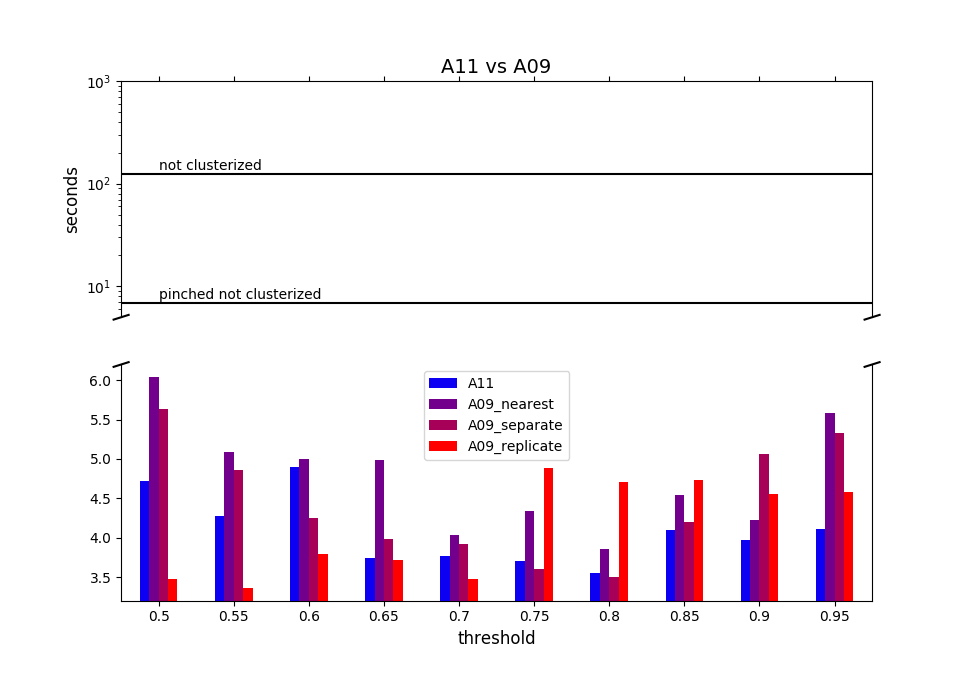
\includegraphics[width=\textwidth, height=7.5cm]{./images/A11-vs-A09-bars.png}
\end{frame}

\begin{frame}{Эксперимент 1 -- скорость получения фрагментов}
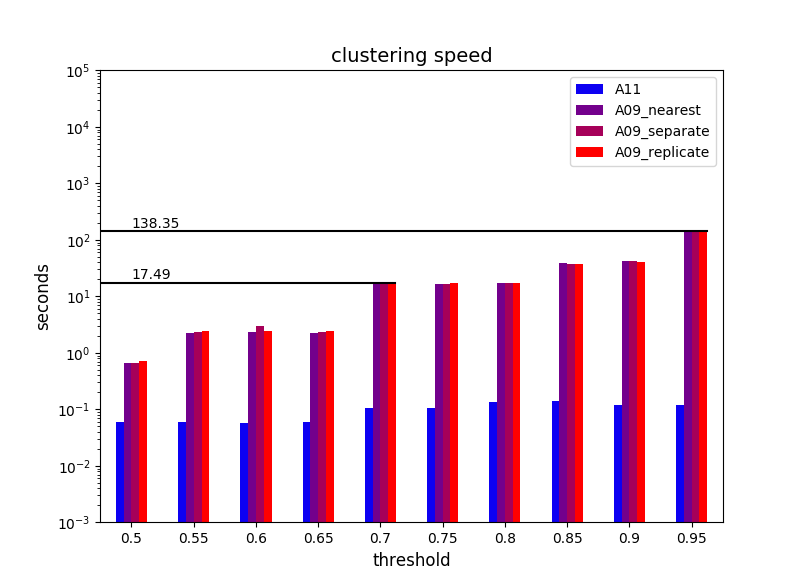
\includegraphics[width=\textwidth, height=7.5cm]{./images/clustering-speed.png}
\end{frame}

\begin{frame}{Эксперимент 2 -- матрицы с фиксированным числом столбцов}

	%\begin{textblock}{5}(0,-1)
	\begin{itemize}
	\item синтетические матрицы
	\item варьирование плотности и размера
	\item $threshold = 0.9$
	\item предел времени выполнения 2 часа
	\end{itemize}
	%\end{textblock}
\vspace*{+0.5cm}\hspace*{-1.5cm}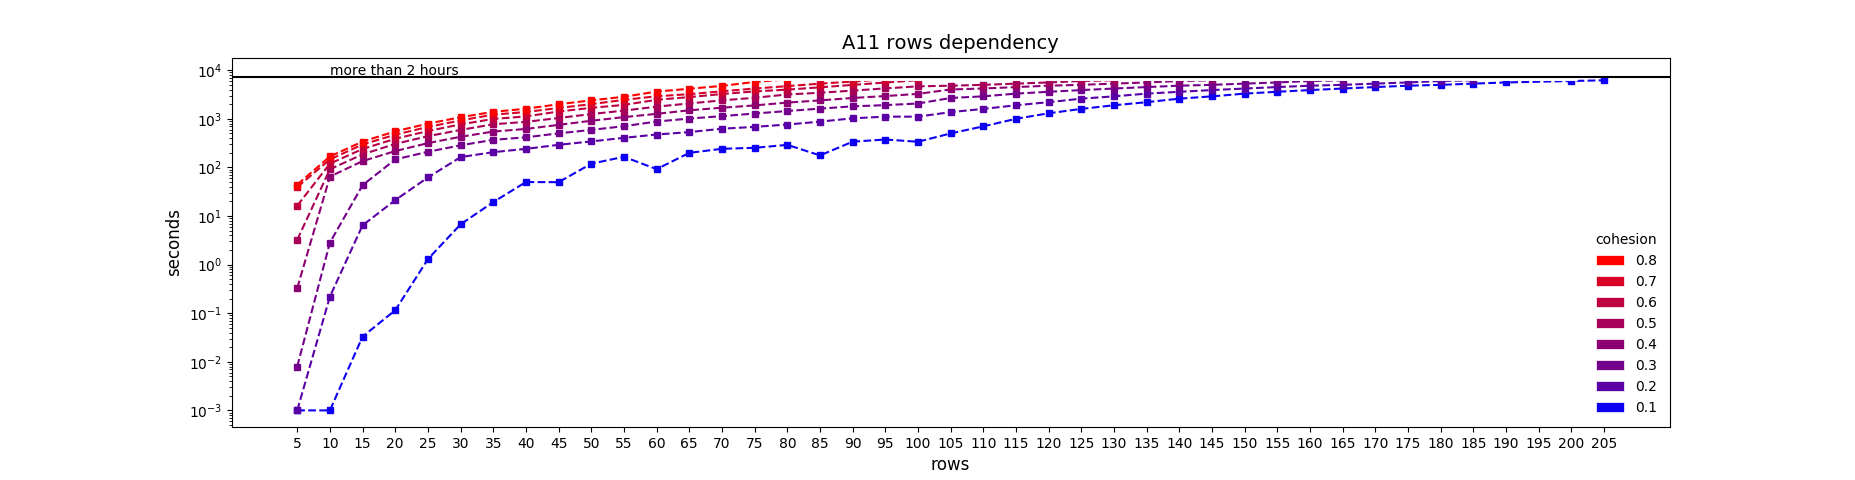
\includegraphics[width=14cm, height=4cm]{./images/A11-X-20.png}
\end{frame}

\begin{frame}{Эксперимент 2 -- матрицы с фиксированным числом строк}
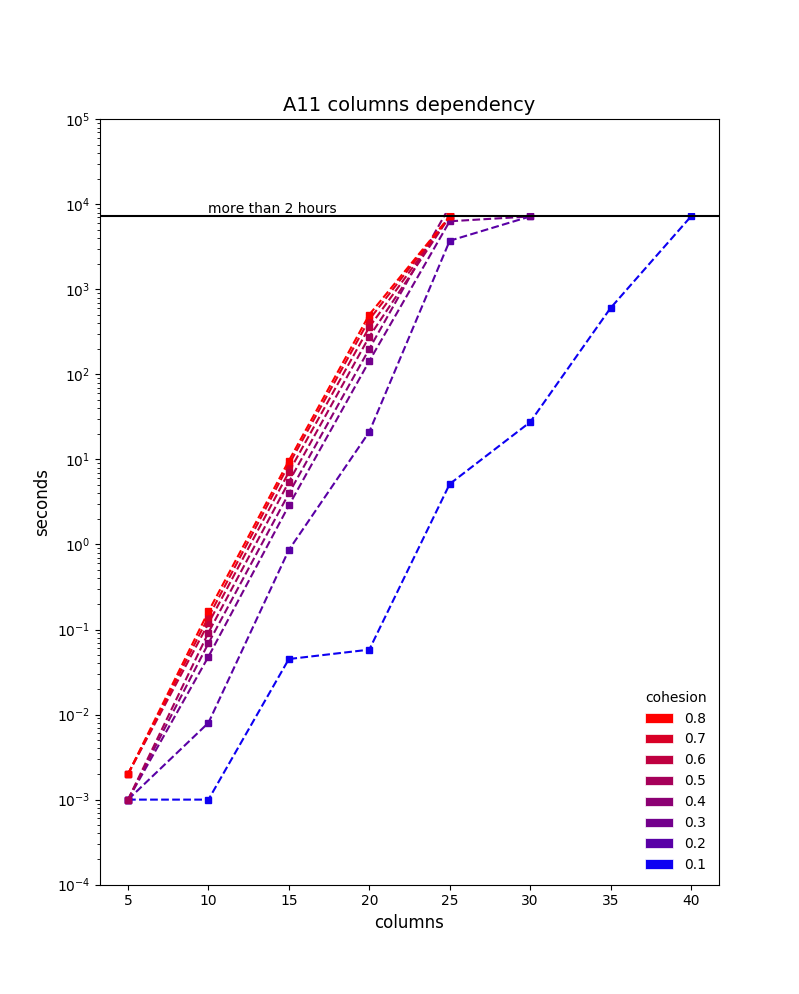
\includegraphics[width=\textwidth, height=7.5cm]{./images/A11-20-X.png}
\end{frame}

\begin{frame}{Эксперимент 2 -- квадратные матрицы}
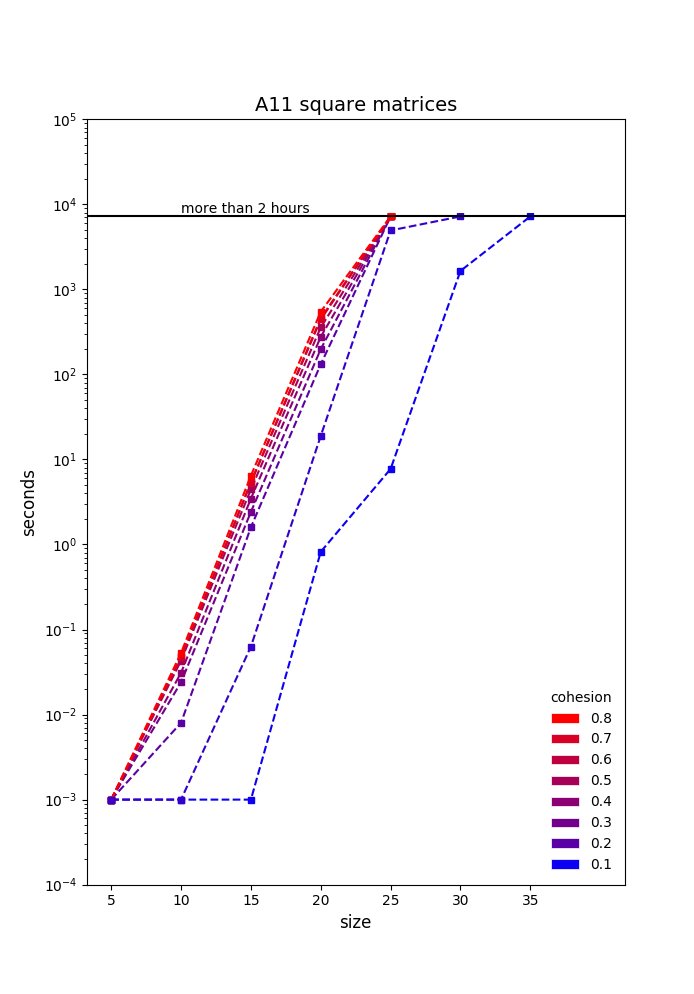
\includegraphics[width=\textwidth, height=7.5cm]{./images/A11-square.png}
\end{frame}

\begin{frame}{Выводы -- 1}
	\begin{itemize}
	\item Фрагментирование повышает производительность
	\item Качество фрагментов зависит от threshold. С этой точки зрения лучше всего работает A09 с replication.
	\item Топ-5 по скорости запросов к фрагментам:\\[0.1cm]
		\begin{tabular}{ | c | c | c | c |}
				\hline
				время & алгоритм & стратегия & threshold \\ \hline
				3.358 & A09      & replicate & 0.55      \\ \hline
				3.472 & A09      & replicate & 0.55      \\ \hline
				3.479 & A09      & replicate & 0.70      \\ \hline
				3.500 & A09      & separate  & 0.80      \\ \hline
				3.553 & A11      &           & 0.80      \\ 
				\hline
		\end{tabular}
	\end{itemize}
\end{frame}

\begin{frame}{Выводы -- 2}
	\begin{itemize}
\item При threshold = 0.7 суммарное время работы всех алгоритмов наименьшее.

\item С данным датасетом A11 сработал почти в 10 раз быстрее, чем A09 вне зависимости от стратегии.

\item Возрастание числа атрибутов замедляет работу алгоритмов быстрее, чем возрастание числа запросов.

\item Наборы фрагментов, производимые алгоритмами, требуют в $1,5-2$ раза больше памяти, чем таблица, состоящая только из используемых атрибутов.

	\end{itemize}
\end{frame}

\end{document}
